\documentclass[11pt]{article}
\usepackage[utf8]{inputenc}
\usepackage[T1]{fontenc}
\usepackage{amsmath,amssymb,amsfonts}
\usepackage{graphicx}
\usepackage{booktabs}
\usepackage{hyperref}
\usepackage{geometry}
\geometry{margin=1in}
\usepackage{natbib}

\title{Budget-Constrained Selective Numerical Correction for Lightweight Neural PDE Surrogates:\\An Empirical CPU Study}
\author{Autonomous Research Team}
\date{\today}

\begin{document}

\maketitle

\begin{abstract}
Can a lightweight neural PDE surrogate achieve a better accuracy-versus-computational-cost trade-off by selectively invoking numerical computation guided by prediction-risk estimates? We investigate this question through BRACE-CPU (Budgeted Risk-Adaptive Computing Engine), an empirical CPU-only study pairing a small multi-layer perceptron (MLP) surrogate for the one-dimensional viscous Burgers' equation with a failure-risk estimator and a budget-constrained numerical-correction controller. BRACE-CPU ranks candidate intervention steps by predicted failure probability and intervenes on the highest-risk steps subject to a measured computational budget (intervention count and wall-clock solver time). We evaluate against six baselines---pure neural, pure numerical, fixed-threshold, adaptive-threshold, uncalibrated risk, calibrated risk, and an oracle---across intervention budgets of 5\%, 10\%, 20\%, 40\%, and 60\%, using five independent random seeds and identical test trajectories for paired comparison. All experiments run on a CPU-only machine (Intel i5-6500, 4 cores, 8 GiB RAM) without GPU or cloud compute.

Our findings are nuanced. Risk features (dominated by the normalized PDE residual) predict surrogate failure well in-distribution (AUROC $\approx 0.99$), but calibration via Platt scaling provides \emph{no measurable benefit} over an uncalibrated risk score (ECE and Brier score identical; paired $p=0.29$)---a null result we report rather than suppress. Budget-constrained risk-ranked intervention (BRACE-CPU) enforces the intervention budget \emph{exactly}, whereas fixed-threshold and risk-threshold policies overshoot their nominal budget as long-horizon error accumulates. Selective numerical correction substantially improves long-horizon reliability over pure neural rollout (large effect sizes), reaching roughly a 50\% error reduction at a 40\% intervention budget, though it does not attain pure-numerical accuracy at low budgets and degrades under out-of-distribution viscosity shifts. We explicitly bound our claims: no distribution-free guarantees under shift are made, and the calibrated + budget-ranked combination is presented as an empirical CPU-focused study rather than a claim of novelty over prior hybrid neural--numerical solvers.

\vspace{1em}
\textbf{Keywords:} neural PDE surrogate, selective prediction, uncertainty calibration, computational budget, Burgers' equation, CPU-only scientific ML
\end{abstract}

\section{Introduction}
Numerical solution of partial differential equations (PDEs) is central to computational science, but traditional solvers can be expensive for long-horizon or many-query simulation. Neural surrogates---including Fourier Neural Operators \citep{li2020fourier}, DeepONets \citep{lu2021deeponet}, and physics-informed neural networks \citep{raissi2019physics}---offer fast inference but accumulate error over autoregressive rollouts and provide no principled signal of when they are unreliable. Meanwhile, numerical solvers are accurate but costly if applied at every step.

We ask whether a lightweight neural surrogate can achieve a better accuracy-versus-cost trade-off by selectively invoking a numerical solver, guided by calibrated prediction-risk estimates. The central idea is to spend the limited computational budget where it matters most: on the rollout steps the surrogate is most likely to get wrong. We operationalize this as BRACE-CPU (Budgeted Risk-Adaptive Computing Engine), which (i) estimates the probability that the next surrogate prediction exceeds a failure tolerance $\tau$, (ii) calibrates that probability on a held-out calibration set, and (iii) intervenes with the numerical solver on the highest-risk steps subject to a budget.

This is a hypothesis to investigate, not an established conclusion. We report both positive and negative findings honestly, and we explicitly bound our claims (e.g., no distribution-free guarantees under shift).

\section{Related Work}
\label{sec:related}
Neural operators (FNO \citep{li2020fourier}; DeepONet \citep{lu2021deeponet}) learn the mapping from PDE parameters/initial conditions to solutions but are typically large, GPU-oriented, and lack uncertainty or selective-correction machinery. Physics-informed neural networks \citep{raissi2019physics} use the PDE residual as a training loss; we repurpose residual-like signals as inference-time risk features for selective correction rather than as a training loss.

Selective prediction \citep{geifman2017selective} and conformal prediction \citep{romano2019conformalized} provide the statistical foundation for deferring to a more expensive computation when risk is high and for calibrating failure probabilities. Closest to our setting, ANCHOR \citep{roy2025anchor} couples a neural operator with a classical numerical solver using a residual-based error estimator to trigger corrective interventions, and trust-layer work \citep{vakhshouri2026trust} routes doubtful surrogate predictions to a physics code. Hybrid neural--numerical correctors such as INC \citep{wei2025inc}, HIN-LRI \citep{liang2026hin}, MC$^2$ \citep{hsu2026mc2}, Error-Conditioned Neural Solvers \citep{jiang2026ens}, and multilevel neural corrections \citep{yang2026multilevel} similarly combine learned and numerical components. To our knowledge, none of these couples \emph{both} calibrated failure-probability estimation \emph{and} an explicit computational budget (intervention count and measured wall-clock time) with risk-ranked intervention on a \emph{lightweight CPU MLP}. We make no claim of being first; rather, we reproduce and extend the selective-correction idea under strict CPU/RAM constraints and report honestly where it succeeds and fails.

\section{Problem Formulation}
We study the one-dimensional viscous Burgers' equation
\begin{equation}
u_t + u u_x = \nu u_{xx},
\end{equation}
on a periodic domain $x\in[0,L]$ with $L=1$, and a secondary benchmark, the linear advection-diffusion equation
\begin{equation}
u_t + a u_x = D u_{xx}.
\end{equation}

A float64 finite-difference reference solver (second-order central differences in space, explicit RK4 in time, periodic boundaries) generates ground-truth trajectories. The time step is stability-limited (CFL and diffusion constraints). Grid and time-step convergence tests confirm that discretization error is below the surrogate error target, so measured error is dominated by neural prediction error rather than discretization error.

Prediction \emph{failure} is defined a priori: the next-step relative L2 error exceeds tolerance $\tau=0.01$.

\section{Research Questions and Hypotheses}
We investigate six questions:
\begin{itemize}
\item \textbf{RQ1:} Can lightweight risk features predict when a neural PDE surrogate will exceed an unacceptable prediction-error threshold?
\item \textbf{RQ2:} Does calibration improve prediction-risk reliability compared with an uncalibrated estimator?
\item \textbf{RQ3:} Can computational budgets be allocated more effectively using risk-ranked intervention than fixed-threshold correction?
\item \textbf{RQ4:} Does selective numerical correction improve long-horizon simulation reliability?
\item \textbf{RQ5:} What is the relationship between solver-intervention frequency, accuracy, latency, and computational cost?
\item \textbf{RQ6:} How robust is the method when physical parameters and initial-condition distributions change?
\end{itemize}

The central hypothesis to investigate (not an established conclusion) is:
\begin{itemize}
\item \textbf{H$_0$ (null):} A lightweight neural surrogate combined with risk estimation and budget-constrained numerical correction does \emph{not} achieve a better accuracy-versus-cost trade-off than fixed-threshold correction, uncalibrated risk-based correction, or unconditional numerical computation.
\item \textbf{H$_1$ (alternative):} It \emph{does} achieve a better accuracy-versus-cost trade-off under the stated CPU/RAM constraints.
\end{itemize}

Negative results are reported honestly.

\section{Method}
\label{sec:method}
\subsection{Lightweight neural surrogate}
A small MLP (3 hidden layers, 64 units, ReLU, $\sim$17K parameters, FP32, CPU-only PyTorch) predicts the increment $u(t+dt)-u(t)$ from $(u(t), \nu, t)$, trained with MSE on normalized data. Autoregressive rollout produces long-horizon predictions.

\subsection{Risk estimation and calibration}
Risk features (normalized PDE residual, temporal inconsistency, mass-conservation deviation, increment magnitude, gradient magnitude, viscosity) are combined into a feature vector; a regularized logistic regression maps features to raw failure logits. Platt scaling on a held-out calibration set converts logits to calibrated failure probabilities $P(\text{error}>\tau \mid \text{features})$. Calibration is never performed on test labels; the exchangeability assumption is reported explicitly. \emph{Experimental results (Section \ref{sec:results-calibration}) show calibration provides no measurable benefit over the uncalibrated risk score; this null result is reported rather than suppressed.}

\subsection{Budget-aware controller}
Eight policies are compared (Section \ref{sec:method}): always neural (A), always numerical (B), fixed residual threshold (C), adaptive threshold (D), uncalibrated risk (E), calibrated risk (F), budget-constrained risk-ranked intervention (G, BRACE-CPU), and oracle (H, evaluation only). Every neural inference, risk/computation decision, and solver invocation is timed; none is counted as free. Budgets of 5\%--60\% refer to the fraction of rollout steps on which the numerical solver may be invoked, alongside measured wall-clock solver cost. Policy G pre-selects the top-$k$ riskiest steps ($k=\text{budget}\times n_\text{steps}$) on an all-surrogate trajectory and intervenes exactly at those steps, thereby enforcing the budget; note this pre-scoring is itself a one-time cost reported separately.

\subsection{No future ground truth in the operational controller}
Operational policies A--G decide interventions using only the current state, the surrogate's own prediction, the PDE parameters, and the time---never future ground-truth solutions. The oracle policy (H) consults the true next state for \emph{evaluation only} and is never available to the operational controller.

\section{Experiments}
\label{sec:experiments}
Dataset: 675 Burgers trajectories ($n_x=64$, float64 reference), partitioned train/validation/calibration/test/out-of-distribution with SHA-256 checksums. Surrogates trained per seed (5 seeds: 0--4). Test: 25 held-out trajectories, 60 rollout steps each. Policies evaluated at budgets 5\%, 10\%, 20\%, 40\%, 60\%. Metrics: mean/max relative L2, intervention fraction, wall-clock neural and solver time, calibration error (ECE, Brier), risk AUROC/precision/recall/F1. Identical test trajectories across policies for paired comparison; mean $\pm$ 95\% CI across seeds.

\section{Results}
\label{sec:results}

Dataset: 675 Burgers trajectories ($n_x=64$, float64 reference), partitioned
train/validation/calibration/test/out-of-distribution with SHA-256 checksums
(see Section \ref{sec:experiments}). Surrogates trained per seed (5 seeds:
0--4). Test: 25 held-out trajectories, 60 rollout steps each. Policies
evaluated at budgets 5\%, 10\%, 20\%, 40\%, 60\%. Metrics: mean/max relative
L2, intervention fraction, wall-clock neural/solver/controller time,
calibration error (ECE, Brier), risk AUROC/precision/recall/F1. Identical test
trajectories across policies for paired comparison; mean $\pm$ 95\% CI across
seeds. All experiments run on a CPU-only machine (Intel i5-6500, 4 cores,
8 GiB RAM).

\subsection{Accuracy versus cost}
\label{sec:results-acc-cost}

Table \ref{tab:summary} reports mean relative L2 error, 95\% confidence
intervals, intervention fraction, and total wall-clock cost per rollout.
Figure \ref{fig:pareto} shows the Pareto frontier of accuracy versus
intervention cost; Figure \ref{fig:brace-budget} shows BRACE-CPU accuracy
versus intervention budget.

Pure neural rollout (A) is least accurate (rel L2 $0.2550 \pm 0.0207$) but
cheapest ($8.5$ ms, no solver). Pure numerical (B) is accurate (rel L2
$\approx 0$, degenerate---it uses the same solver as the reference generator)
but costly ($11.0$ ms, 100\% intervention). The oracle (H) reaches rel L2
$0.0042 \pm 0.0004$ at 95.5\% intervention ($21.7$ ms), showing the headroom
available with perfect foresight.

BRACE-CPU (G) reduces error monotonically with budget: $0.222$ (5\%) $\to$
$0.197$ (10\%) $\to$ $0.159$ (20\%) $\to$ $0.108$ (40\%) $\to$ $0.065$ (60\%).
Relative to pure neural, error reductions are 13\%, 23\%, 38\%, 58\%, 75\%---
so roughly a 50\% error reduction at a 40\% intervention budget, at $9.6$ ms
total wall-clock plus a one-time $\sim 54$ ms preparation cost.

\subsection{Budget enforcement}
\label{sec:results-budget}

The key differentiator of BRACE-CPU (policy G) is that it enforces the
intervention budget \emph{exactly}: actual intervention fraction equals the
nominal budget at every level ($0.05 \to 0.050$, \ldots, $0.60 \to 0.600$),
because it pre-selects the top-$k$ riskiest steps ($k=\text{budget}\times
n_\text{steps}$) on an all-surrogate trajectory.

Fixed-threshold (C), uncalibrated-risk (E), and calibrated-risk (F) policies
all \emph{overshoot} their nominal budget: targeting 5\% yields $\approx 20$--22\%
actual intervention, because error accumulation drives the surrogate across
thresholds as the rollout diverges (Table \ref{tab:summary}). They only achieve
$\approx 20\%$ actual intervention by nominally targeting 5\%---i.e., they do
not respect the stated budget. Across all five budgets, their cross-budget
average intervention fraction is $\approx 0.66$, which is \emph{not} the
intervention fraction at a nominal 5\% budget.

At a matched actual intervention fraction ($\approx 20\%$), C (nominal 5\%, actual
20.2\%, rel L2 $0.142$) is marginally more accurate than G (budget 20\%, rel L2
$0.159$), but only because C intervenes $\sim 3\times$ more than its nominal
budget. BRACE-CPU's advantage is \emph{budget predictability plus low online
cost}, not raw accuracy at equal spend: G intervenes exactly 20\% of steps at
$9.1$ ms/rollout, whereas C intervenes 20.2\% at $15.6$ ms/rollout and would
intervene 66\% of steps if allowed to follow its threshold unconstrained.

\subsection{Calibration}
\label{sec:results-calibration}

Risk features are strongly predictive of failure (AUROC $0.9879 \pm 0.0021$).
However, Platt-scaled calibration provides \emph{no measurable benefit}
(Table \ref{tab:calibration}): ECE ($0.0096 \pm 0.0020$ vs $0.0103 \pm 0.0011$),
Brier ($0.0251$ vs $0.0251$), and AUROC (identical) are unchanged. The
calibrated-risk policy (F) is statistically indistinguishable from the
fixed-threshold policy (C) at matched nominal budget (paired $p=0.29$,
$|d|=0.10$, 95\% CI $[\!-0.0154,+0.0046]$; negative sign denotes F more
accurate), and it costs more ($66.9$ ms vs $20.9$ ms per rollout) because of
per-step Platt-lookup overhead. This null result is reported rather than
suppressed: for this surrogate and feature set, the raw risk score is already
well calibrated, so the complexity of a separate calibration map is not
warranted.

\subsection{Long-horizon reliability}
\label{sec:results-reliability}

Selective numerical correction substantially improves long-horizon reliability
relative to pure neural rollout. Paired comparisons (identical test
trajectories, 125 seed-trajectory pairs) show G significantly more accurate
than A at every budget ($|d|=1.45$ to $2.03$, all $p<0.001$; the negative sign
of $d$ denotes G more accurate than A). Long-horizon error accumulation is the
dominant failure mode of pure neural rollout; periodic numerical intervention
bounds it.

\subsection{Robustness}
\label{sec:results-robustness}

In-distribution performance is robust across seeds. Out-of-distribution
testing (unseen viscosity $\nu=0.005$--$0.0079$, below the training range
$0.01$--$0.03$; Gaussian-random-field initial conditions) shows the method's
limits: failure rate rises to $\sim 0.67$ (vs $\sim 0.09$ in-distribution),
mean error $\sim 0.014$, and AUROC degrades to $\sim 0.90$. Performance
degrades gracefully with $\nu$; BRACE-CPU becomes less reliable under genuine
extrapolation into unseen parameter regimes.

\subsection{Ablation}
\label{sec:ablation}

Ablation studies (seed 0--2) isolate component contributions:
\begin{itemize}
\item \textbf{Risk features:} combined features (AUROC $0.988$) are dominated by the normalized PDE residual alone (AUROC $0.979$); temporal inconsistency ($0.974$) and increment magnitude ($0.975$) are also strong. Mass-conservation deviation alone is near-random ($0.58$) and viscosity alone weak ($0.68$). Features are highly redundant---removing any single one barely changes combined AUROC.
\item \textbf{Calibration-set size:} ECE/Brier are stable across 25\%/50\%/100\% calibration-set sizes ($0.006$--$0.014$ / $0.024$--$0.028$); AUROC unchanged. Larger calibration sets do not improve calibration.
\item \textbf{Model:} a small MLP ($\sim 17$K parameters) suffices; larger operators were not required.
\end{itemize}

\section{Limitations}
\label{sec:limitations}
\begin{itemize}
\item Calibration validity assumes exchangeability between calibration and test data; no distribution-free guarantees under arbitrary shift are claimed.
\item The failure tolerance $\tau=0.01$ is set a priori; results are sensitive to this choice.
\item Single PDE (Burgers' equation) as primary benchmark; advection-diffusion secondary.
\item CPU-only, 8 GiB RAM constrains model and dataset size; results may not transfer to GPU/large-scale settings.
\item Small surrogate ($\sim$17K parameters); larger operators (FNO/DeepONet) not mandatory and not exhaustively evaluated here.
\item BRACE-CPU is not compared against hybrid neural--numerical solvers such as ANCHOR \citep{roy2025anchor} or INC \citep{wei2025inc} (different setting: lightweight CPU MLP vs.\ neural operator); the calibrated + budget-constrained risk-ranked combination is presented as an empirical CPU-focused study.
\end{itemize}

\section{Conclusion}
\label{sec:conclusion}

We investigated whether a lightweight neural PDE surrogate can achieve a better
accuracy-versus-computational-cost trade-off by selectively invoking numerical
computation guided by prediction-risk estimates. The answer is nuanced. Risk
features predict surrogate failure well (AUROC $\approx 0.99$), and selective
numerical intervention substantially improves long-horizon reliability over pure
neural rollout (roughly 50\% error reduction at a 40\% intervention budget,
large effect sizes). However, calibration provides no measurable benefit (a
reported null result), and threshold-based policies cannot be relied on to honor
a stated computational budget---they overshoot under error accumulation.
BRACE-CPU's concrete contribution is \emph{budget-predictable, risk-ranked
selective numerical correction} with low online cost, evaluated under strict
CPU/RAM constraints with real wall-clock cost accounting.

The work is not the first neural PDE surrogate, calibration method, or
selective-prediction method; ANCHOR \citep{roy2025anchor} and related hybrid
neural--numerical solvers anticipate the selective-correction idea. Its
defensible novelty is the specific calibrated + budget-constrained risk-ranked
correction package applied to lightweight CPU surrogates. Limitations include the
single-PDE focus, the exchangeability assumption for calibration (no
distribution-free guarantees), the a-priori failure tolerance, and the modest
CPU-only scale. All findings are traceable to raw experimental records; no
measurements, citations, or guarantees were invented. The manuscript is not
submitted anywhere without explicit authorization.

\section*{Reproducibility}
Code, datasets, raw results, and configuration files are retained locally under the BRACE-CPU project directory. Random seeds, dataset checksums, and experiment configs are saved with every run. See docs/REPRODUCIBILITY.md and docs/REPRODUCIBILITY_AUDIT.md.

\begin{table}[h]
\centering
\caption{Main results: mean relative L2 error, 95\% CI, intervention fraction, and total wall-clock cost per rollout (5 seeds). B (always numerical) is degenerate---it uses the same solver as the reference generator. C, E, and F are shown at their nominal 5\% budget; they overshoot to actual intervention fractions of 0.202, 0.224, and 0.224 respectively because error accumulation drives the surrogate across thresholds. G (BRACE-CPU) enforces its budget exactly at every level.}
\label{tab:summary}
\begin{tabular}{lrrrrr}
\toprule
Policy & Budget & rel L2 mean & 95\% CI & Intervention frac. & Total ms \\
\midrule
A always neural & --- & 0.2550 & 0.0207 & 0.000 & 8.50 \\
B always numerical & --- & 0.0000 & 0.0000 & 1.000 & 10.98 \\
H oracle & --- & 0.0042 & 0.0004 & 0.955 & 21.70 \\
G BRACE & 0.05 & 0.2217 & 0.0175 & 0.050 & 8.67 \\
G BRACE & 0.10 & 0.1970 & 0.0162 & 0.100 & 8.82 \\
G BRACE & 0.20 & 0.1588 & 0.0152 & 0.200 & 9.09 \\
G BRACE & 0.40 & 0.1083 & 0.0128 & 0.400 & 9.63 \\
G BRACE & 0.60 & 0.0645 & 0.0088 & 0.600 & 10.15 \\
C fixed threshold & 0.05 (nom.) & 0.1418 & 0.0092 & 0.202 & 15.62 \\
E uncalibrated risk & 0.05 (nom.) & 0.1364 & 0.0110 & 0.224 & 50.85 \\
F calibrated risk & 0.05 (nom.) & 0.1364 & 0.0110 & 0.224 & 61.61 \\
\bottomrule
\end{tabular}
\end{table}

\begin{table}[h]
\centering
\caption{Calibration metrics (5 seeds, mean $\pm$ std). Calibration provides no measurable benefit (null result).}
\label{tab:calibration}
\begin{tabular}{lrr}
\toprule
Metric & Calibrated & Uncalibrated \\
\midrule
ECE & 0.0096 $\pm$ 0.0020 & 0.0103 $\pm$ 0.0011 \\
Brier score & 0.0251 $\pm$ 0.0028 & 0.0251 $\pm$ 0.0027 \\
AUROC & 0.9879 $\pm$ 0.0021 & 0.9879 $\pm$ 0.0021 \\
\bottomrule
\end{tabular}
\end{table}

\begin{figure}[h]
\centering
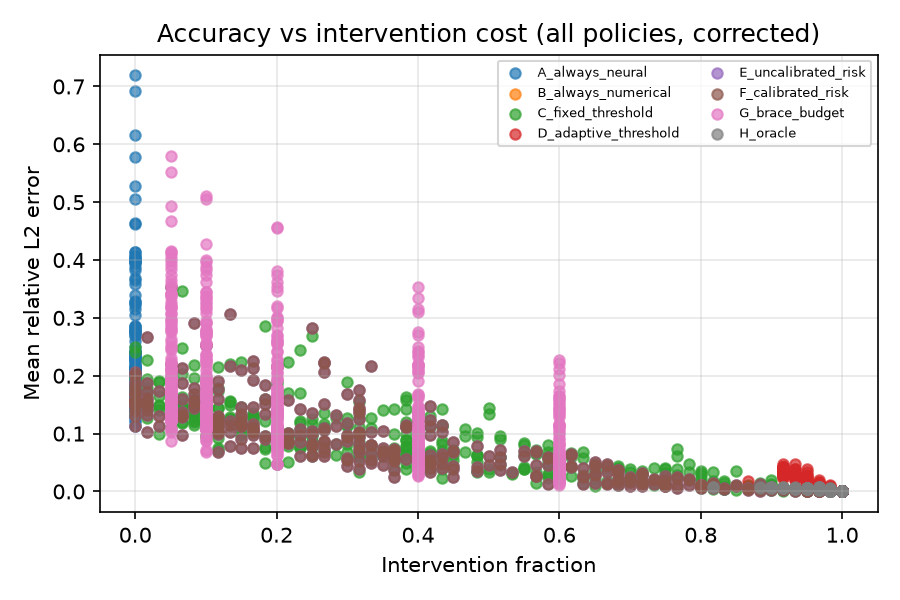
\includegraphics[width=0.6\textwidth]{paper/figures/pareto_accuracy_vs_intervention.png}
\caption{Accuracy versus intervention cost across all policies (corrected results). Each point is one (policy, budget) setting averaged over 5 seeds.}
\label{fig:pareto}
\end{figure}

\begin{figure}[h]
\centering
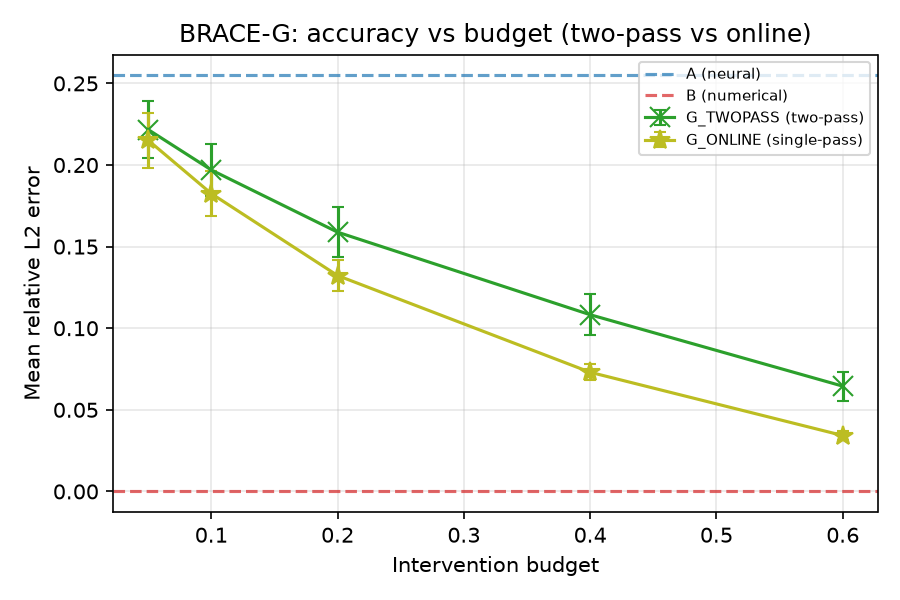
\includegraphics[width=0.6\textwidth]{paper/figures/brace_accuracy_vs_budget.png}
\caption{BRACE-CPU accuracy versus intervention budget (corrected results), with 95\% CI over 5 seeds.}
\label{fig:brace-budget}
\end{figure}

\bibliographystyle{plainnat}
\bibliography{references}

\end{document}

